\documentclass[12pt]{article}
\usepackage{jcappub}
\usepackage{amsmath}
\usepackage{graphicx}
\usepackage{xcolor}
\usepackage[normalem]{ulem}
\usepackage{mathtools} %For summations with limits
\usepackage{multicol} %For multiple columns
\setlength{\columnsep}{1cm}


\title{The Distribution of Vacua in Random Landscape Potentials}

\author{Low Lerh Feng,}
\author{Shaun Hotchkiss}
\author{and Richard Easther}

\emailAdd{lerh.low@auckland.ac.nz}
\emailAdd{s.hotchkiss@auckland.ac.nz}
\emailAdd{r.easther@auckland.ac.nz}

\newcommand{\re}[1]{\textcolor{blue}{[{\bf RE}: #1]}}
\newcommand{\lfl}[1]{\textcolor{red}{[{\bf LL}: #1]}}
\newcommand{\SH}[1]{\textcolor{brown}{[{\bf SH}: #1]}}
\newcommand{\sh}[1]{\textcolor{brown}{#1}}
\newcommand{\LFL}[1]{\textcolor{red}{#1}}


\affiliation{Department of Physics,\\ University of Auckland, \\Private Bag 92019,\\ Auckland, New Zealand}

\abstract{ Landscape cosmology posits the existence of a convoluted, multidimensional, scalar potential -- the  ``landscape'' -- with vast numbers of metastable minima. The huge number of minima supported by landscape potentials motivate arguments that landscape cosmology reduces tuning problems associated with a small but non-zero vacuum energy by providing a framework in which anthropic or ``environmental'' selection is plausible. Random matrices and random functions in many dimensions can be used to discuss  conceptual issues associated with landscape scenarios; here we explore the number ofminima as a function of and vacuum energy in an $N$-dimensional Gaussian random potential. We derive a probability density for the density of minima in $N$ dimensions, showing that after rescalings its properties are fully defined by $N$ and a single free parameter. This gives us $P(\Lambda)$, the probability density function of vacuum energies in these scenarios. \re{little more to come}}

\begin{document}

\maketitle

\section{Introduction}

Over the last two decades cosmology has developed in apparently paradoxical directions. Observationally, the rise of ``precision cosmology'' makes it possible to measure key parameters to within a few percent, setting stringent tests for the detailed evolutionary narrative given by concordance $\Lambda$CDM cosmology\cite{Planck2018,DES}. Conversely, theoretical investigations of both slow-roll inflation and string theory along with a non-zero dark energy density motivates  theoretical investigations of multiverse-like scenarios. In particular, studies of stochastic inflation \cite{Linde1986,Adshead2007} suggest that the mechanism that produces astrophysical density perturbations could also support {\em eternal inflation\/}, generating infinite numbers of  {\em pocket universes\/} \cite{Guth2001}. Likewise, studies of flux compactified string vacua points to a possible  {\em landscape\/} \cite{Susskind2003} or {\em discretuum\/} \cite{Bousso2000}   of vacua within the theory. These developments open the door to anthropic explanations of the non-zero vacuum energy density, insofar as a value that was  exactly zero could have been more plausibly explained by an unknown symmetry. 

Stochastic (or eternal) inflation implies the existence of a multiverse composed of many pocket universes, but this does not require that the ``low energy" (i.e. LHC scale) physics or vacuum energy differs between pockets:  the naive quadratic inflation model is potentially eternal, but has a unique vacuum.  By contrast, landscape models have multiple vacua which can, in principle, be populated by stochastic inflation or tunneling. The string landscape, built on the plethora of flux-stablilsed vacua that exist inside Calabi-Yau spaces, is well-known but  is not necessarily a unique realisation of this scenario. The complexity of the landscape  and the vast number of vacua it supports is the basis of its purported explanatory power: the number of vacua is almost uncountably large (e.g. $10^{500}$ or greater \cite{Douglas2003}) and any value of the vacuum energy can thus conceivably be realised within it. 
 
The detailed properties of any possible landscape are almost entirely unknown.  However, an intriguing approach to landscape scenarios is to strip them down to their barest essence -- by realising multiverse cosmology within a {\em random\/} multidimensional ($N\sim100$ or more) potential of interacting scalar fields.\footnote{Random is used here in the  context of random function theory \cite{GRF1, GRF2, GRF3}.  We refer to random functions rather than random fields, the nomenclature often seen in the mathematical literature, to avoid confusion with the individual scalar fields that are coupled by the potential.}  In this approach the ``large $N$'' properties of the multidimensional landscape actually provides leverage that can be used to develop an understanding of its properties. The first steps in this direction were taken by Aazami and Easther \cite{Aazami2006}, investigating ensembles of Hessian matrices describing extrema in a random landscape. At  a minimum in the landscape the eigenvalues of the Hessian are all positive. For simple random matrix distributions eigenvalues are likely to be evenly distributed between positive and negative values with fluctuations away from this situation being strongly suppressed at even moderate values of $N$, suggesting that the number of minima is super-exponentially smaller than the number of saddles. However, the individual entries of Hessians matrices of random functions are correlated and therefore not drawn from identical, independent distributions,\cite{Battefeld2012,Easther2016} violating a common premise of simple random matrix theory and making minima more probable that this initial analysis suggested.  This overall approach has now been widely pursued and extended in a number of directions \cite{Easther2006, Frazer2011, Henry2009, Marsh2013, Agarwal2011,Yang2012,Masoumi2016,Yamada2018} This line of inquiry has also motivated studies of the properties of random matrices and random functions at large $N$.\cite{Bray2007,Dean2008,Majumdar2009,Bachlechner2014,Battefeld2012,Fyodorov2013,Masoumi2017} Similar mathematical problems arise in statistical mechanics, string theory, and complex dynamics.\cite{Fyodorov2004,Douglas2004,Douglas2006,Fyodorov2007,Fyodorov2012,Fyodorov2018,Ros2019}

%The theory of inflation is the current best explanation for certain perplexing observations of the Universe, such as the monopole problem, horizon problem, and flatness problem. Inflation is thought to be caused by a scalar field, but the exact nature of this field is shrouded in unknowns. The simplest possibility is a one-dimensional scalar field analogous to the gravitational potential; however multidimensional scalar fields are also possible. In particular, string theory predicts the existence of a highly complex, $O(100)$ dimensional scalar field known as the \emph{landscape}. The string landscape is so complex that quantitative predictions are hard to extract; as a result, most studies of the landscape assume it is a Gaussian random field

In the conventional picture of the multiverse, a pocket universe traces out a path in the landscape. Regions of the landscape where the gradient of the potential in the ``downhill'' direction(s) is small will yield slow-roll inflation. If the landscape is bounded below typical semi-classical trajectories terminate in a local minimum, whose value fixes the apparent cosmological constant. Moreover, bubbles of space can tunnel between minimum, eventually populating all possible minima in the landscape.  The {\em measure problem\/} for the multiverse is notoriously complex but in this scenario we can use the known properties of Gaussian random fields to estimate $P(\Lambda)$ -- the distribution of possible cosmological constants -- as a function of the dimensionality of the landscape.  This probability is of course distinct from the likelihood that an arbitrary observer will measure a given value of $\Lambda$ as this will be convolved with complex anthropic considerations. However, we will show that for a nontrivial volume of parameter space,  $\int_0^\infty d\Lambda P(\Lambda) \ll 10^{-M}$  where $M$ is a number of ${\cal{O}}(100)$, so the corresponding landscape thus possesses no metastable solutions with  positive vacuum energy. Moreover, we show that in scenarios where positive minima are expected to be extremely rare or nonexistence, the smallest second derivatives of the potential at these rare minima will be much smaller than those found near typical minima, make these scenarios more likely to support quintessence solutions. 


\re{more on physics} 
 -- it is still unclear whether any specific stringy construction  realises  the $SU(3) \times SU(2) \times U(1)$ gauge group of the Standard Model.  More recently the Swampland Conjecture suggests that all stable minima of the theory might actually be ``underwater'' \cite{Agrawal2018},  located at negative values of $\Lambda$. If true, this would appear to require that the cosmological dark energy was underpinned by dynamical quintessence-like evolution.  


We proceed from an $N$-dimensional generalisation of the Kac-Rice formalism \cite{Kac1943,Rice1945} and the  machinery developed and summarised by Bond, Bardeen, Kaiser and Szalay  \cite{BBKS} for studying the statistics of Gaussian random functions in three dimensions. This yields $N$-dimensional integral expressions for the proportion of minima that will have a given value of the potential, $V$. At $N=2$ the full integral can be evaluated analytically; at $N \lesssim 10$ we can directly compute the full integrals numerically; and for $N \lesssim 100$ we evaluate Gaussian approximations to the underlying integrals . The Gaussian approximations are tested against the exact numerical result for $N <10$ where they match closely. These techniques can be generalised to other, more complex questions about trajectories in these potentials, and give information about the ``shapes'' of minima which may inform analyses of tunnelling and inflation. We show that $P(\Lambda)$, the probability density function for the vacuum energy, depends on the dimensionality $N$ and a single free parameter for a Gaussian random landscape, and calculate how $P(\Lambda)$ varies with $N$. \re{Eigenvalues; motivation for working numerically}

\section{Random Potentials in $N$ Dimensions}

%\sh{\sout{We begin by developing an $N$-dimensional analogue of the treatment of three dimensional random functions due to Bardeen, Bond, Kaiser and Szalay (henceforth BBKS) \cite{BBKS}, generalising their derivation and keeping their notation as far as possible.}}\SH{We're no longer following the notation and we say the rest in the paragraph just before this, in the introduction}.

We treat the potential energy function $V({\vec{\phi}})$ as a Gaussian random function over an $N$-dimensional field space. We wish to examine minima and saddles, therefore we require the probability density for the value of the potential itself and the values of its derivatives, $\eta_i = \partial V/\partial \phi^i$ and $\zeta_{ij}=\partial^2 V/\partial \phi^i\partial \phi^j$ at individual points in this field space. These variables can be grouped together into a vector ${\bf y} = [V,\eta,\zeta]$. In $N$ dimensions ${\bf y}$ has $\mathcal{N}=1+N+(N^2+N)/2$ independent components via $V$, $\eta$ and $\zeta$ respectively. $V$ is a Gaussian random function, this means that the variables in ${\bf y}$ are described by a multivariate Gaussian distribution. A general multivariate Gaussian distribution with $\mathcal{N}$ independent variables has the form \re{should that be a curly $N$ on the $2 \pi$ }
  %
\begin{equation} \label{MultivariateGaussian}
\begin{split}
P({\bf y})d^\mathcal{N}{\bf y} &= \frac{e^{-Q}}{[(2\pi)^N \mathrm{det}(M)]^{1/2}} d^\mathcal{N}{\bf y} \, ,\\
Q &\equiv \frac{1}{2} \sum_{i,j}^\mathcal{N} \Delta y_i (M^{-1})_{ij} \Delta y_{j} \, .\\
\end{split}
\end{equation}
%
Here $\Delta y_i$ is the difference between the actual value and the mean value, i.e. $\Delta y_i \equiv y_i - \langle y_i \rangle$, and $M$ is the \emph{covariance matrix}, 
%
\begin{equation}
M_{ij} \equiv \langle \Delta y_i \Delta y_j \rangle.
\end{equation}
%
Averages denoted by $\langle \,\,\rangle$ are ensemble averages. We further assume that $\langle V\rangle = \langle \eta\rangle = \langle \zeta\rangle = 0$.\footnote{$\langle V\rangle=0$ can always be obtained by a constant shift in the definition of $V$. $\langle \eta \rangle = 0$ and $\langle \zeta\rangle = 0$ can be enforced by assuming $V$ is statistically isotropic in field space. An interesting path for future work would be to examine our results without this assumption of statistical isotropy.} Therefore the probability density only depends on the covariance matrix, $M$, and its inverse.

We next introduce the field space power spectrum, $P$, of the random function $V$, which will be useful for writing $M$ in a concise form. We define it here to be the Fourier transform of the correlation function of $V$, i.e.
%
\begin{equation}\label{powspec}
\langle V(\vec{\phi}_1) V(\vec{\phi}_2) \rangle = \xi(|\vec{\phi}_1-\vec{\phi}_2|)= \frac{1}{(2\pi)^N} \int d^Nk e^{i \vec{k} \cdot (\vec{\phi}_1-\vec{\phi}_2)} P(k).
\end{equation}
%
We have assumed $V$ is statistically homogeneous and isotropic in field space, therefore $\xi$ depends only on $|\vec{\phi}_1-\vec{\phi}_2|$ and  $P$ depends only on the magnitude of the Fourier coordinate $k$.\footnote{We work in a field space basis where the field space metric is Euclidean.} The moments of the power spectrum are defined to be
%
\begin{equation} \label{moments}
\sigma_n^2 = \frac{1}{(2\pi)^N}\int d^Nk (k^{2})^n P(k)
\end{equation}
%
This gives $\sigma_0^2=\xi(0)=\langle V^2 \rangle$.

We can differentiate equation \eqref{powspec} and then set $\vec{\phi}_1 = \vec{\phi}_2$ to get

\begin{align*}
\langle \eta_{i}\eta_{j}\rangle &= \frac{1}{(2\pi)^N} \frac{\partial}{\partial \phi_1^i}\frac{\partial}{\partial \phi_2^j} \int d^Nk e^{i \vec{k} \cdot (\vec{\phi}_1-\vec{\phi}_2)} P(k)\bigg{|}_{\vec{\phi}_1=\vec{\phi}_2}\\
&= \frac{1}{(2\pi)^N}\int d^Nk (k^i k^j) P(k)
\end{align*}
%
The integrand on the RHS is an odd function of both $k^i$ and $k^j$, therefore the integral over all $\vec{k}$ is zero unless $i=j$. Furthermore, because $k^2 = \sum_i k_i^2$,  $\sum_i \langle \eta_{i}\eta_{i}\rangle = \sigma_1^2$. We have assumed the field is statistically isotropic and thus $\langle \eta_{i}\eta_{i}\rangle=\langle \eta_{j}\eta_{j}\rangle$, meaning $\langle \eta_{i}\eta_{i}\rangle=\sigma_1^2/N$ and $\langle \eta_{i}\eta_{j}\rangle=\delta_{ij}\sigma_1^2/N$.

%\begin{align*}
%\langle \eta_{\alpha,i}\eta_{\beta,j}\rangle = K \delta_{\alpha,\beta}\delta_{ij} &\rightarrow \delta_{ij}\langle \eta_{\alpha,i}\eta_{\beta,j}\rangle = NK \delta_{\alpha,\beta}=\sigma_1^2\\
%&\rightarrow K = \frac{1}{N}\sigma_1^2
%\end{align*}

A similar analysis holds for the second derivatives $\zeta_{ij}$, and will yield the rest of the elements of the covariance matrix. In terms of the moments of the power spectrum these are:
%
\begin{equation} \label{corr}
\begin{split}
\langle VV \rangle &= \sigma_0^2 \\
\langle\eta_i\eta_j\rangle &= \frac{1}{N}\delta_{ij}\sigma_1^2 \\
\langle V\zeta_{ij}\rangle &= -\frac{1}{N}\delta_{ij}\sigma_1^2 \\
\langle\zeta_{ij}\zeta_{kl}\rangle &= \frac{1}{N(N+2)}\sigma_2^2(\delta_{ij}\delta_{kl}+\delta_{il}\delta_{jk}+\delta_{ik}\delta_{jl})
\end{split}
\end{equation}
%
and all other correlations are zero. For $N=3$ this reduces to equation A1 of \cite{BBKS} (hereafter called BBKS). 

%We define the following vector\SH{This small passage is the only time the notation $\alpha$ is used. I think we can get away without introducing it. I think in general the way BBKS goes from $F$ at different points in space to $F$, $\eta$ and $\xi$ is confusing and we can make it a bit clearer here if we want}:

%\begin{equation}
%\begin{split}
%\alpha = \{F,\eta_1,\eta_2,\ldots,\xi_{11},\xi_{22},\ldots,\xi_{NN},\xi_{N-1,N},\xi_{N-2,N},\ldots,\xi_{1N},\xi_{N-2,N-1},\\
%\ldots\xi_{1,N-1},\ldots,\xi_{12}\}
%\end{split}
%\end{equation}

%\noindent With this choice for $\alpha$ (equivalent to $\Delta y$ in Eq. \ref{MultivariateGaussian}), the covariance matrix $M_{ij}\equiv\langle\alpha_i\alpha_j\rangle$ and its inverse $K \equiv M^{-1}$ takes the following general form\SH{I guess this result comes from Mathematica? There must be a way of simplifying the $K_{\xi_{ij}\xi_{kl}}$ terms into one expression using $\delta_{ij}$ etc, like with $M$. Actually, this $K$ seems to never be used so I'm not sure we need to write it down. If we want to write out the inverse in all detail we should do it in terms of the variables we eventually use (i.e. $x_i$)}:

%\begin{align*}
%K_{F, F} &= \frac{\sigma_2^2}{\sigma_0^2\sigma_2^2-\sigma_1^4} \\
%K_{F, \xi_{ij}} &= \frac{\sigma_1^2}{\sigma_0^2\sigma_2^2-\sigma_1^4} \\
%K_{\eta_i,\eta_j} &= \frac{N}{\sigma_1^2}\\
%K_{\xi_{ii},\xi_{ii}} &=  \frac{N(N+2)}{\sigma_2^2} \\
%K_{\xi_{ij}, \xi_{ij}} &= \frac{N\sigma_0^2\sigma_2^2-(N+2)\sigma_1^4}{2(\sigma_1^4\sigma_2^2-\sigma_0^2\sigma_2^4)}, (i\neq j)\\
%K_{\xi_{ii}, \xi_{jj}} &= \frac{(N(N+1)-2)\sigma_1^4 - N(N+1)\sigma_0^2\sigma_2^2}{2(\sigma_1^4\sigma_2^2-\sigma_0^2\sigma_2^4)}, (i \neq j)\\
%\end{align*}

%\noindent and all other terms are zero\SH{Are there some $\delta_{ij}$ terms missing in the 2nd and 3rd lines above?}. The probability density of $\alpha_i$ is, from Eq. \ref{MultivariateGaussian}\SH{This is just eq. 2.2 repeated with $\alpha$ instead of $y$, I think there is a way of expressing all of this without so many introduced variables like $y$ $\alpha$ that are used only once each. I don't we've ever explicitly said we're considering functions/fields where $\langle F\rangle=0$ either, which we've assumed in order to write this equation.}.

%\begin{equation} \label{ProbDistrib}
%p(\alpha_i)=\frac{1}{(2\pi)^{N/2}\sqrt{\mathrm{det}M}} e^{-\frac{1}{2}\alpha K \alpha}
%\end{equation}
%
%We can usually ignore the constant prefactor since we will primarily be concerned with ratios of probabilities.
This covariance matrix is far from diagonal; and our analysis will be facilitated if we use a basis that is as close to diagonal as possible. The $\eta_i$ variables are already diagonal, as are the $\zeta_{ij}$ terms with $i\neq j$ but the $\zeta_{ii}$ variables are correlated to each other, and also  to $V$. We look for a set of $N$ linear combinations of these $N$ variables that is diagonal, choosing,
\begin{align}
\label{BasisTransform}
x_1 &= -\frac{1}{\sigma_2}\sum_i\zeta_{ii} \nonumber \\
x_n &= -\frac{1}{\sigma_2}\sum_{i=1}^{n-1}\zeta_{ii}-(n-1)\zeta_{nn},\,\, (2\leq n \leq N) \, .
%\sigma_2x_3 &= -(\xi_{11}+\xi_{22}-2\xi_{33})\\
%\sigma_2x_4 &= -(\xi_{11}+\xi_{22}+\xi_{33}-3\xi_{44})\\
%\ldots
\end{align}
%
The $x_n$ here are analogous, but not identical, to BBKS's $x, y, z$. Following BBKS, we also rescale $V$, introducing $\nu = V/\sigma_0$. With this choice of basis in equation \eqref{corr} become
%
\begin{eqnarray}
  \langle\nu^2\rangle &=& 1 \nonumber\\
  \langle x_1^2\rangle&=&1 \\
  \langle\nu x_1\rangle &=& \gamma \nonumber\\
  \langle x_n^2 \rangle &=& \frac{2n(n-1)}{N(N+2)},\,\, (2\leq n \leq N) \nonumber
\end{eqnarray}
%
\noindent where $\gamma = \sigma_1^2/(\sigma_2 \sigma_0)$. The only non-diagonal correlation left is between $\nu$ and $x_1$.

The $Q$ factor in equation \eqref{MultivariateGaussian} becomes
%
\begin{equation} \label{Q}
\begin{split}
2Q = \nu^2 + \frac{(x_1-\gamma \nu)^2}{1-\gamma^2}+\sum_{n=2}^N\frac{N(N+2)}{2n(n-1)}x_n^2 + \frac{N \pmb{\eta}\cdot \pmb{\eta}}{\sigma_1^2} + \sum_{i,j;i > j}^N\frac{N(N+2)(\zeta_{ij})^2}{\sigma_2^2}
\end{split}
\end{equation}
%
This is the equivalent of BBKS equation (A4) for $N$-dimensions. Note that the first two terms remain constant for all $N$, but the remaining terms are $N$ dependent.  

Equations \eqref{Q} and \eqref{MultivariateGaussian} give, in as diagonal a form as possible, the full probability density function for the function, $V$, and its first two derivatives at an arbitrary point in field space. We are interested in characterising the distribution of \emph{minima} of $V$, and begin by looking at the number density of extrema, i.e. points where $\eta=0$. BBKS \cite{BBKS} (section III a) show how to obtain the number density of extrema from the probability density (for $N=3$ ).  BBKS consider a field $F$ in Euclidean space with position vector ${\bf r}$, whereas we have an $N$-dimensional function $V$ with coordinates $\phi$. \SH{We could reproduce the working in BBKS if we want, it seems a bit weird to reproduce everything above and then not reproduce this, but this doesn't change for ND vs 3D.}\re{I think it would be nice} 
%
\begin{equation}
n_{\rm ext}(\phi) \,\,{\rm d}^N \phi= |{\rm det}\,\, \zeta(\phi)| \delta^{(N)}\left[ \eta(\phi)\right] {\rm d}^N \phi.
\end{equation}
%
The number density of extrema, $n_{\rm ext}(\phi)$, is itself a random variable. However, we will work with the \emph{expected} number density, which is simply the ensemble average of $n_{\rm ext}$, or
% 
\begin{equation} \label{NumberDensity}
\langle n_{\rm ext}(\phi)  \rangle= \int |{\rm det}\,\, \zeta(\phi)| P(V,\eta=0,\zeta)dV d\zeta
\end{equation}
where for notational convenience we have dropped the ${\rm d}^N \phi$ from each side.

Finally, we need to restrict this integral to count the extrema that are also local minima. It is easiest to do this by considering the eigenvalues, $\lambda_i$ of the Hessian of the landscape $-\zeta$\SH{What convention do we want to use here for the sign?}\re{haven't tried to sort this, but isn't the Hessian usually just the second derivatives (outside of random function theory), so let's use that?}  and restricting them to be negative.\footnote{Note there is an alternative convention where the eigenvalues \sh{are defined with the opposite sign, in which case} \emph{positive} \sh{eigenvalues} correspond to \sh{minima} \re{cite places where this is used}}  The Hessian is  symmetric by definition. We can further rotate it such that it is diagonal, in which case the diagonal elements are its eigenvalues.  In 2D and 3D, the Jacobian of the transformation matrix can be calculated explicitly as $d \zeta = \prod_{i \neq j}^N |\lambda_i - \lambda_j|(\prod_k d\lambda_k) d \Omega$, where ``$d\Omega$'' represents the $(N^2-N)/2$-dimensional integral measure of the set of rotation angles. The same result holds in $N$ dimensions.\footnote{A proof in $N$ dimensions is given in section V of \cite{Easther2016}, generalising the 3D  BBKS result. \re{can we just say what the typos are?}} The function $V$ and its derivatives are statistically isotropic. Therefore each set of rotation angles is as probable as any other, and the integral over all the rotation angles must give just a constant.   After this rotation $\zeta_{ii}=-\lambda_i$, $\zeta_{ij}=0$ and $|{\rm det} \zeta| = \prod_i |\lambda_i|$. and the factor $|\rm{det} \zeta(\phi)|$ in Eq. \ref{NumberDensity} can be expressed as $A \prod_i |\lambda_i| \prod_{i \neq j}^N |\lambda_i - \lambda_j|(\prod_k d\lambda_k)$, where $A$ is a constant.

 


 We now have  the ingredients we  need, but  also enforce an ordering on the eigenvalues to avoid dealing with a multimodal integrand.  We define  $\lambda_1 \leq \lambda_2 \leq \lambda_3 \ldots \leq 0$ so our boundary conditions become $x_1\leq x_N\leq x_{N-1} ... \leq x_2 \leq 0$, and the mapping between $\lambda_i$ and $x_i$  follows from Equation~\ref{BasisTransform}. This gives significantly simpler boundary conditions than our earlier choices for diagonalising the covariance matrix and yields the following expression for the expected number density of minima 
%
\begin{equation} \label{DensityOfPeaks}
\langle n_{{\rm min}} \rangle = A \int_{\lambda_1 \leq \lambda_2 \leq \lambda_3 \ldots \leq 0} G \times e^{-Q} d\nu  \left(\prod_n dx_n\right)
\end{equation}
%
\noindent where $G$ has the form\footnote{$G$ can also be expressed in terms of $x_n$ using the inverse transform of Eq. \ref{BasisTransform}.}

\begin{equation}
G = \left(\prod_{i}^{N} \lambda_i \right)\left(\prod_{i<j} |\lambda_i-\lambda_j|\right),
\end{equation} 
%
$Q$ is given by Eq. \ref{Q} and the constant factor $A$ has absorbed by Jacobian. More generally, we can view the expression
%
\begin{equation}
{\cal L}(\lambda_1,\cdots, \lambda_N; V, \gamma) = \left(\prod_{i}^{N} \lambda_i \right)\left(\prod_{i<j} |\lambda_i-\lambda_j|\right) e^{-Q}
\end{equation} 
%
as an unnormalised probability density that gives the (relative) likelihood of finding a minimum at which the landscape has a $V$, and the Hessian matrix has eigenvalues $\lambda_i$ as a function of the single independent variable $\gamma$. This expression is exact;  we immediately see that the prefactor to the exponential enforces a variant of {\em eigenvalue repulsion\/} \re{cite RMT literature; in general you can have a symmetric matrix with degenerate eigenvalues}, in that the likelihood of finding a minimum with near-identical $\lambda_i$ is vanishingly small. 



\section{Landscape Heuristics}

Our  overall goal is to understand $P(\Lambda)$, the probability density of energy densities (ie the values of $V(\phi)$) at the minima of a Gaussian random landscape. In particular, we are interested in the proportion of  minima with $V > 0$, which is given by\footnote{We assumed earlier that $\langle V \rangle = 0$. In principle, one could consider an ``offset'' landscape, which consisted of a Gassian random field with zero mean, plus a constant, such that $\langle V \rangle \neq 0$ but we do not explore this here.}
\begin{equation} \label{PminIntegral}
  P(\Lambda >0| N,\gamma) =  \frac{\int^\infty_0 d\nu \int_{\lambda_1 \geq \lambda_2 \geq \lambda_3 \ldots \geq 0} G \times e^{-Q} \prod_n dx_n}{\int^\infty_{-\infty} d\nu \int_{\lambda_1 \geq \lambda_2 \geq \lambda_3 \ldots \geq 0} G \times e^{-Q} \prod_n dx_n}
  \end{equation}
 %
 and any specific $P(\Lambda)$ can be computed by dropping the integral over $\nu$ and setting $\nu=\Lambda$ in the numerator. 
 %
%
This integral depends on the value of $Q$ (Eq. \ref{Q}) and therefore on the moments of the power spectrum $\sigma_0, \sigma_1$,  and $\sigma_2$, through the single parameter $\gamma$. The allowed range of this variable is $0<\gamma<1$ because $0<\sigma_1^2<\sigma_0\sigma_2$. \SH{could add proof if we wanted}\re{since we have it}


Broadly speaking, the overall distribution $P(\Lambda | N,\gamma)$ moves to lower values as $N$ and $\gamma$ are increased;  representative results for moderate $N$ are shown in Figure~\ref{distributions}. Moreover, as $\gamma$ increases, the width of the distribution contracts. Consequently, we will find that when $\gamma$ is close to unity and $N \gtrsim {\cal{O}}(10^2)$, $P(\Lambda >0)$ can be almost arbitrarily small, as we quantify below. 


\begin{figure}
  \centering
  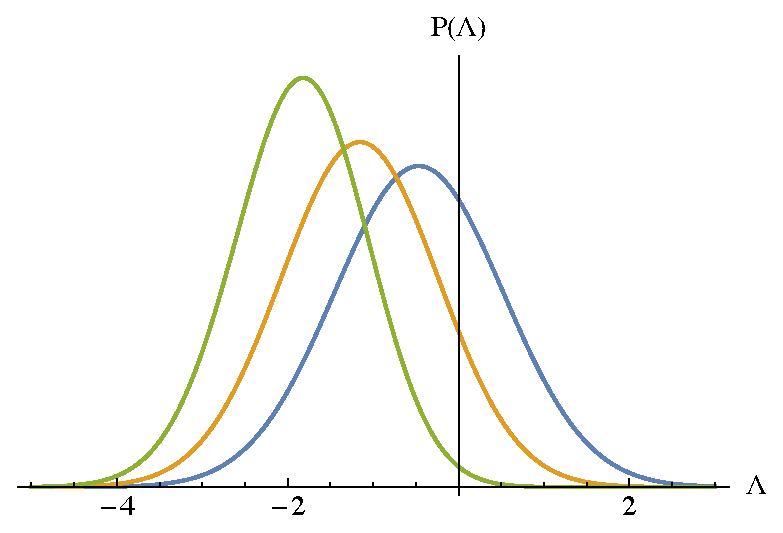
\includegraphics[width=0.45 \linewidth]{PLam_gamma.eps}  \hfill
  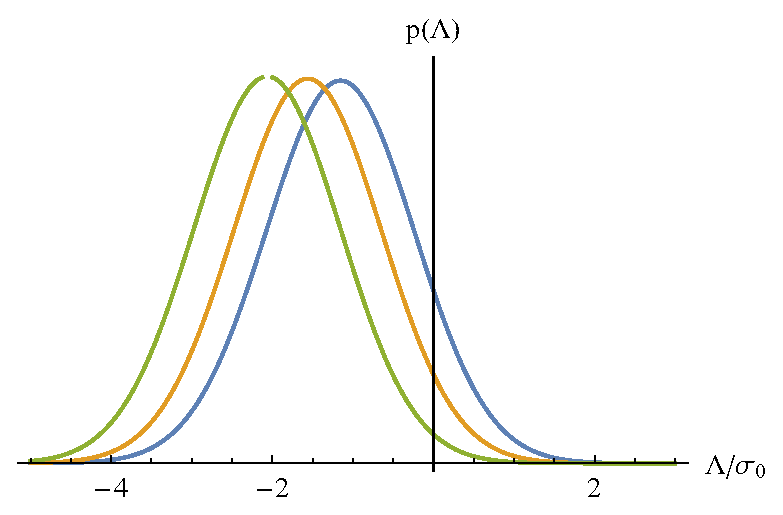
\includegraphics[width=0.45 \linewidth]{PLam_N.eps}
  \caption{[Left] $P(\Lambda)$ for $\gamma = 0.2$, $0.5$ and $0.8$ and [Right] $P(\Lambda)$ for $N=3$, $5$ and $8$. The distribution moves leftward with increasing $N$ and increasing $\gamma$. The results were obtained by numerically evaluating the full integral for $P(\Lambda)$.  }
  \label{distributions}
  \end{figure}

%def of gamma, and power spectrum
This dependence on $\gamma$ and $N$ can be understood qualitatively via the expressions for $\sigma_2$ for the probability density. Via its definition, $\sigma_2$ increases as the range of $k$ over which the spectrum $P(k)$  is nontrivial  increases, and $\gamma$ will correspondingly decrease. Conversely, when $\gamma$ is close to unity, the power spectrum is peaked over a small range of $k$ and the random function is dominated by modes with a narrow band of wavelengths.  At small $\gamma$ the spectrum of $V(\phi)$ thus has power over a wide range of scales. This points to the presence of significant ``ripples'' on top of  larger-scale structure in $V(\phi)$, which  produce local minima even $V(\phi)$ is relatively large,  as illustrated in Fig~\ref{examples1}.  Similarly, while the second derivatives of a random function are correlated, at values of $V$ large enough for minima are rare, increasing $N$  increases the number of directions that must have an unlikely value of $\zeta_{ii}$. 

We can likewise see $N$-dependence semi-quantitatively by noting that the number of terms in polynomial $G$ grows rapidly with $N$, so the full probability density at minima prefer larger magnitude eigenvalues, $|\lambda_i|$. Since $x_1$ is the sum of the eigenvalues, as its magnitude grows the $(x_1-\gamma \nu)^2$ term in $Q$ also grows. For minima, $x_1<0$, therefore large $|x_1|$ makes it less likely to find minima with $\nu >0$ (or $\nu <0 $ for maxima).  \re{but the expected value of $x_1^2$ is unity, via 2.7?. Not sure this is nailed.}


\begin{figure}
  \centering
    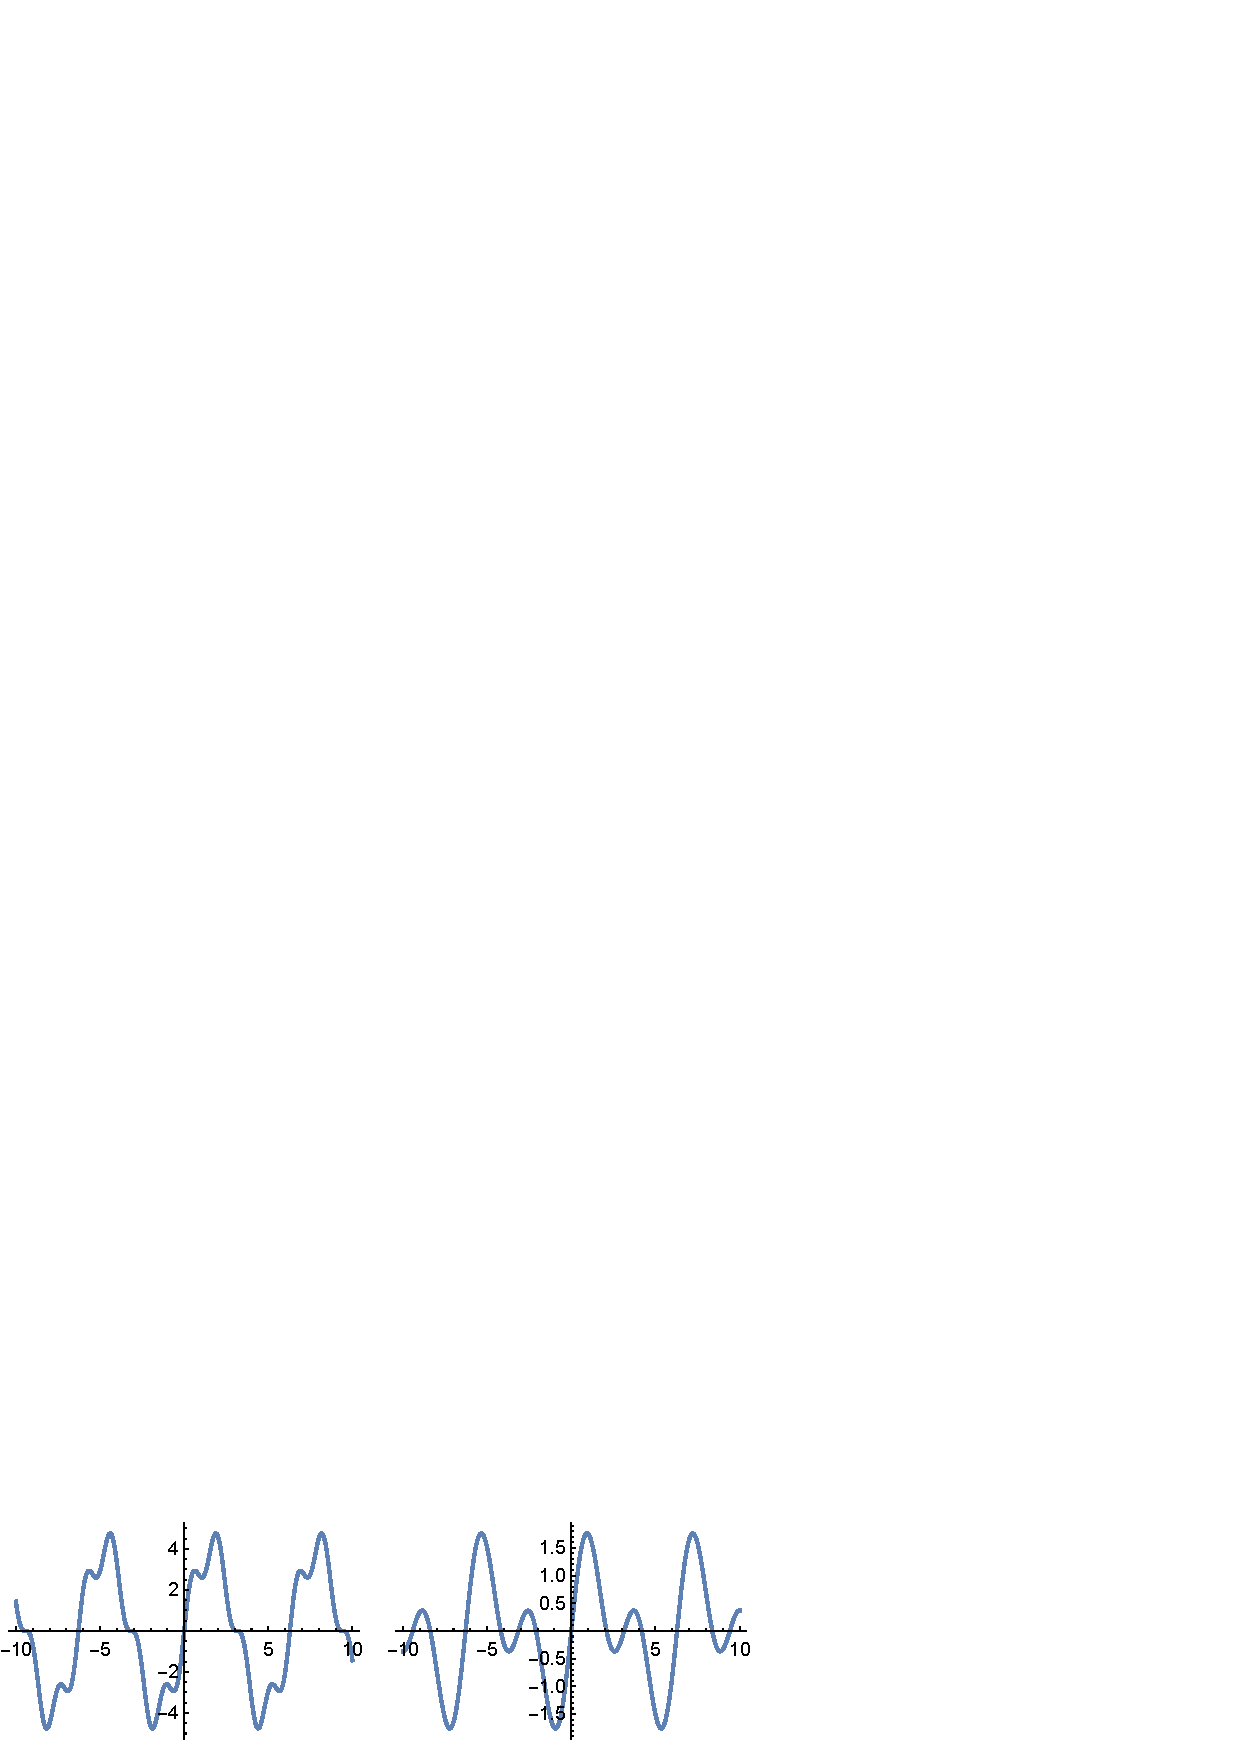
\includegraphics[width=\linewidth]{TwoSigmas.png}
  \caption{Illustrative realisations of 1D functions. The left figure has a small $\gamma$ and power over a greater range of scales, allowing minima (maxima) to appear in significant numbers above (below) zero. When $\gamma$ is large (right figure) the spectrum is dominated by  a smaller range of modes, and most minima are low-lying. \SH{y-axis on LHS and RHS are subtly different}}
  \label{examples1}
\end{figure}

 % integrals over V
Note that we can perform the integrals over $\nu$ in Eq. \ref{PminIntegral} analytically. The only dependence of the integrand on $\nu$ is via the first two terms of $Q$, which are independent of $N$. Consequently, we can write the denominator of Eq. \ref{PminIntegral} as 
%
\begin{eqnarray}
\nonumber {\rm denom} &=&
\int^\infty_{-\infty} d\nu \int_{\lambda_1 \geq \lambda_2 \geq \lambda_3 \ldots \geq 0} G \times e^{-Q} \prod_n dx_n \\ 
\nonumber &=&  \int_{\lambda_1 \geq \lambda_2 \geq \lambda_3 \ldots \geq 0} f(x_1, x_2 \ldots) \prod_n dx_n \int^\infty_{-\infty} d\nu \,\exp\left(-\frac{\nu^2}{2}- \frac{(x_1- \gamma \nu)^2}{2(1-\gamma^2)}\right)\\
&=& \sqrt{2\pi (1-\gamma^2)}  \int_{\lambda_1 \geq \lambda_2 \geq \lambda_3 \ldots \geq 0} f(x_1, x_2 \ldots) \prod_n dx_n\exp\left(-\frac{x_1^2}{2}\right) \, .
\end{eqnarray}
% 
where $f$ is implicitly defined.  Similarly, the $\nu$ integral in the numerator can be performed to yield an error function. However, the general expressions are intractable. 
%
%\begin{figure}
%  \centering
%    \includegraphics[width=\linewidth]{PVaryingWithN.png}
%  \caption{A plot showing the value of $P(V>0|{\rm min})$ as a function of $N$ with $N\le10$, for $\gamma$ values $\frac{1}{5}, \frac{1}{3.5}$ and $\frac{1}{2}$ from top to bottom.\SH{Title needs changed}}
%  \label{gamma}
%\end{figure}

 
Given the dependence of $P(\Lambda|N,\gamma)$ on $N$ and $\gamma$ it is clear that as these variables increase $P(\Lambda>0|N,\gamma)$ will involve the increasingly rare tail of an increasingly narrow distribution. Figure~\ref{N6} shows $P(\Lambda>0)$ as a function of $\gamma$ for values of $N$ that are small enough for the relevant integrals to be evaluated numerically, and we see that positive minima grow far less likely as $N$ and $\gamma$ increase. 



\begin{figure}
  \centering
  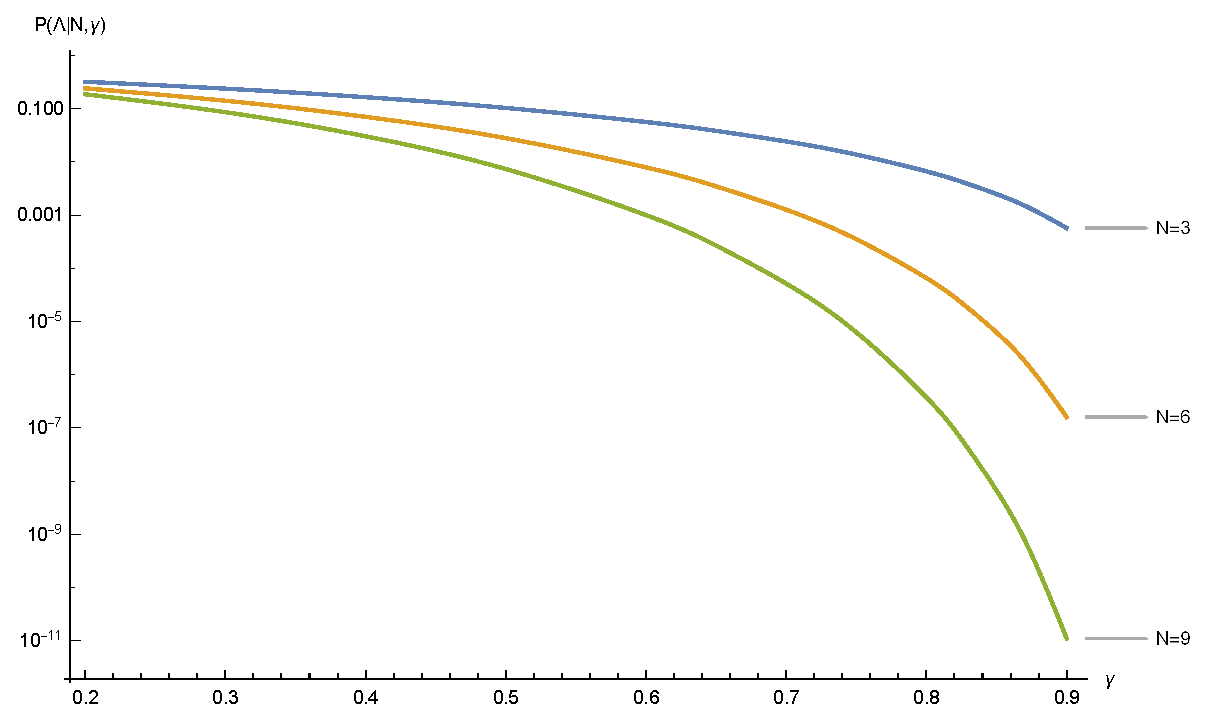
\includegraphics[width=.6 \linewidth]{N369.eps}
  \caption{The probability that a given minimum has $V > 0$ as a function of $\gamma$, for $N=3, 6, 9$. We see that all the heuristics are obeyed: the probability decreases with $N$, and  $\gamma$.}
  \label{N6}
  \end{figure}


   


 

\section{Gaussian Landscapes: Evaluating $P(\Lambda)$} \label{PeakNumbers}

We now turn to the problem of evaluating $P(\Lambda|N,\gamma)$  for more general parameter values. Many and perhaps all of the following calculations could be performed using analytical techniques in a large-$N$ limit. However,  as we are particularly interested in scenarios involving extreme tails of  the probability distribution we will focus on quasi-numerical strategies for obtaining quantities of interest. Moreover, we are  not necessarily working at ``large'' $N$; given the inherently speculative nature of this investigation, there are few  grounds for specifying likely values of $N$;  $N\sim{\cal O}(10^2)$ is not unreasonable, but we cannot necessarily rely on results that may only hold well as $N\rightarrow \infty$. 

That said, for $N>10$, direct calculation becomes very resource-intensive. To proceed, we approximate the full integrand as a Gaussian; fixing $\gamma$ and find the values of $x_n$ that maximize the integrand in Eq. \ref{DensityOfPeaks}, or 
%
\begin{align*}
\begin{split}
\langle n_{\rm min}(\nu)\rangle d\nu &=A\int_{\lambda_1 \geq \lambda_2 \geq \lambda_3 \ldots \geq 0} e^{\mathrm{log}G-Q} \prod_n dx_n d\nu\\
&\approx \int_{-\infty}^{\infty} \exp\left(-\frac{1}{2}\sum_{l,m}x_lH_{lm}x_m\right)  \prod_n dx_n d\nu \\
&= \sqrt{\frac{(2\pi)^N}{\mathrm{det} H(\nu)}}d\nu
\end{split}
\end{align*}
%
\noindent where $H_{lm}$ is the Hessian \sh{of the integrand with respect to the $x_n$ variables} at the peak.
\begin{figure} 
  \centering
  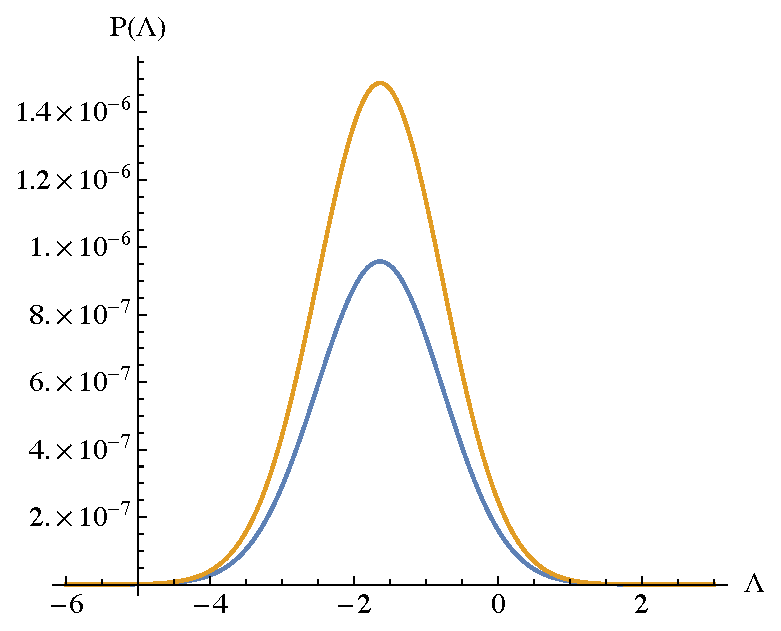
\includegraphics[width=.3 \linewidth]{PLam_approx.eps} \hfill
   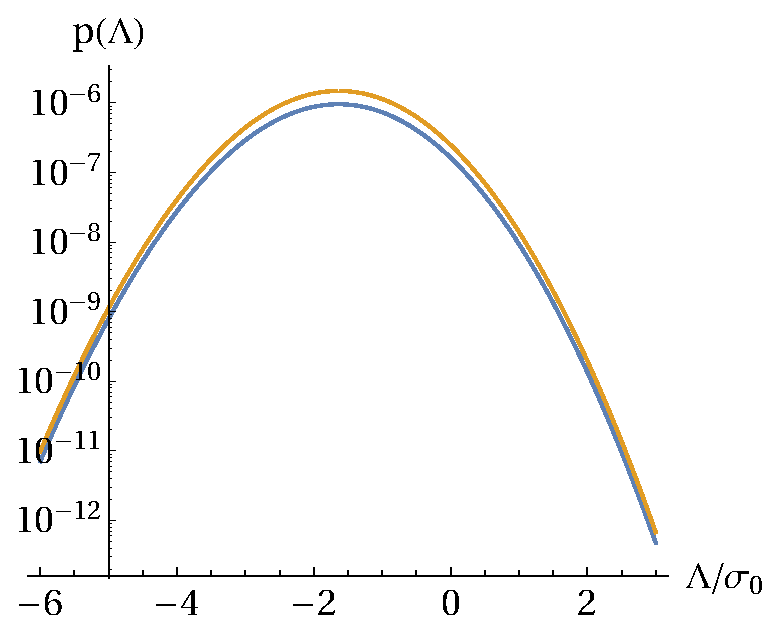
\includegraphics[width=.3 \linewidth]{PLam_approx_log.eps} \hfill
    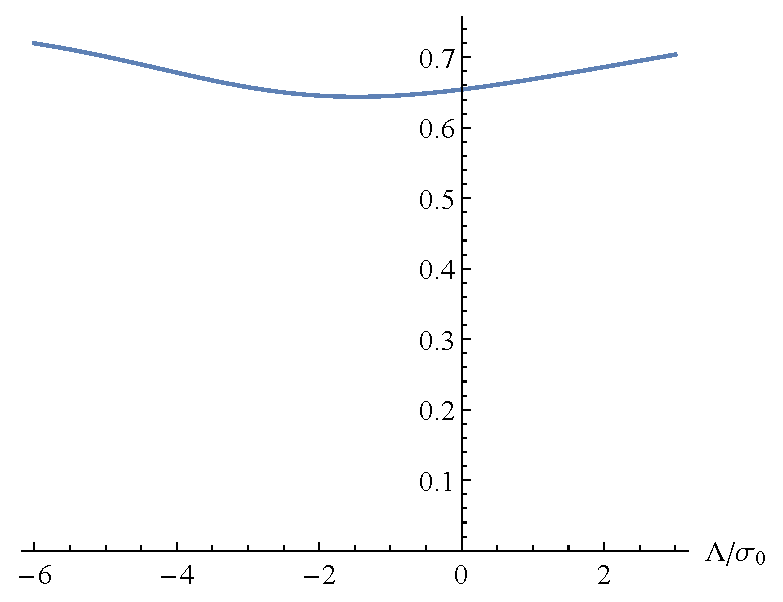
\includegraphics[width=.3 \linewidth]{PLam_ratio.eps}
  \caption{  
  A comparison of the unnormalised exact $P(\Lambda)$ with the Gaussian approximation, for $\gamma=0.6$ and $N=4$. The left and middle plots show the exact result and the Gaussian approximation, on linear and logarithmic axes; the ratio of the two is show on the right. The Gaussian approximation always  over-estimates the integral, but the ratio is roughly independent of $\Lambda$ and remains close to unity. }
  \label{Comparison}
\end{figure}

It turns out that the numerical location of the peak can be obtained fairly simply for $N\lesssim 200$, which will be sufficient for our purposes.\footnote{All numerical results in this paper are obtained using Mathematica. We note that the computational efficiency of the calculations can depend strongly on apparently small tweaks in their implementation.} A representative comparison between the Gaussian approximation and the exactly evaluated integral is shown in Figure~\ref{Comparison}, and we see that it is sufficiently accurate for our purposes. In particularly, for fixed $N$ and $\gamma$ the discrepancy between the exact result and the approximation depends very weakly on $\Lambda$, so  the normalised results will be highly accurate.  
\SH{We could include here the comparison to $(N-1)^\alpha$ to show we understand why the gaussian approximation misses. We could also use the $(N-1)^\alpha$ corrected Gaussian approximation as the default if we want. Finally, I think we could do with a more thorough examination of when/where this approximation works and where it doesn't, as a function of $N$ and $\gamma$.} \re{include to agree  this could use more discussion, but not to go overboard} 

\begin{figure} 
  \centering
  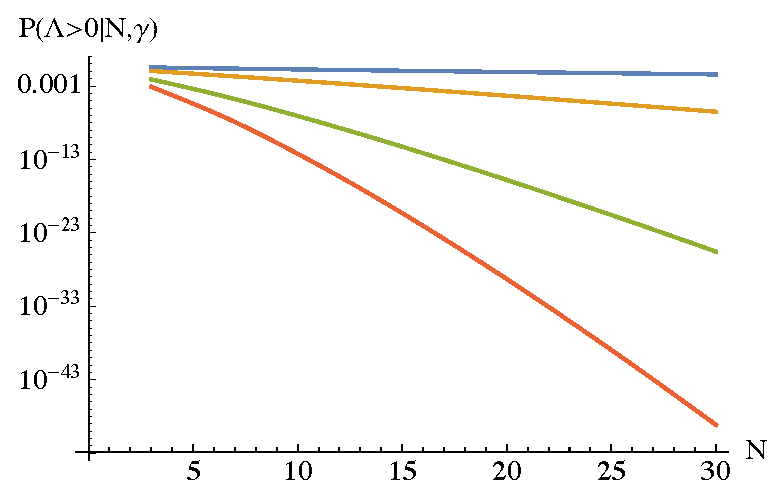
\includegraphics[width=.6 \linewidth]{pwithN.eps}
  \caption{The probability that a given minimum has $\Lambda>0$, as a function of $N$ for $\gamma=0.2$, $0.5$, $0.8$ and $0.9$ (top to bottom) calculated using the Gaussian approximation. }
  \label{PVaryingWithNGaussian}
\end{figure}
  
In  Figure~\ref{PVaryingWithNGaussian} we show $P(\Lambda>0|N,\gamma)$ as a function of $N$ for several values of $\gamma$, given by Equation~\ref{PminIntegral}. We use the Gaussian approximation for the integrals over the $x_i$; in the numerator we compute the final integral over $\nu$ by evaluating at multiple, evenly spaced values of $\nu > 0$  and then performing a simple numerical integral. We see that the logarithms of $P(\Lambda>0|N,\gamma)$ are linear with $N$, but the constant of proportionality increases rapidly as $\gamma$ approaches unity; for $N=30$ and $\gamma = .9$ only 1 in $10^{50}$ minima in the landscape will have a positive cosmological constant. 

In practice, when $\Lambda>0$ is effectively in the right-hand tail of $P(\Lambda)$,  the value of $P(\Lambda=0|N,\gamma)$ is a reliable proxy for $P(\Lambda>0|N,\gamma)$. In the tail of the distribution,  $P(\Lambda|N,\gamma)$ will decrease significantly between $\nu=0$ and $\nu=1$, so $P(\Lambda=0|N,\gamma)$ will always overestimate $P(\Lambda>0|N,\gamma)$. However, because we have normalised $\nu$, the factor between the $\Lambda=0$ and $\Lambda>0$ case will not depend strongly on $N$ or $\gamma$ and is typically less than a factor of $10$. In other circumstances this would be a poor approximation, but here our focus is effectively on the logarithms of very small numbers, so this factor can be safely ignored. 

\begin{figure} 
  \centering
  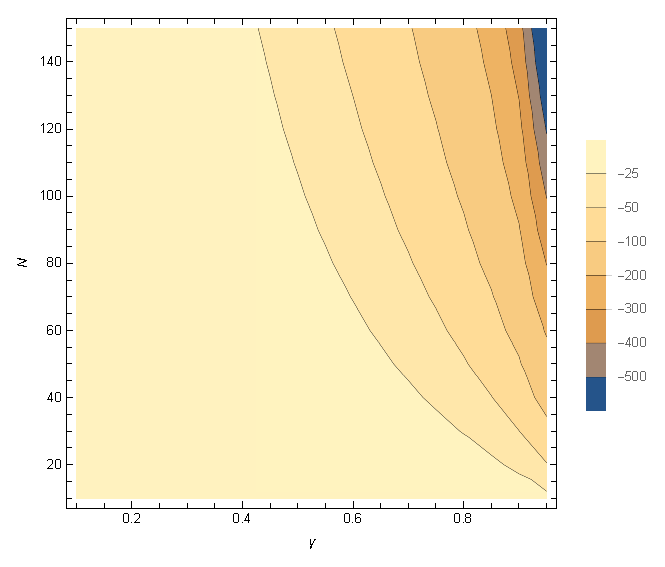
\includegraphics[width=.6 \linewidth]{histo.eps}
  \caption{The contour plot displays $P(\Lambda =0 |N,\gamma)$. Contours are at $\log_{10}(P(\Lambda =0 |N,\gamma)) = -25$, -50, -100, -200, -300, and  -400.  We see that for $N \sim 100$ there are significant regions of parameter space for which $P(\Lambda =0 |N,\gamma)$ is vastly less than unity. }
  \label{fullcontourplot}
\end{figure}

Figure~\ref{fullcontourplot} displays  $P(\Lambda =0 |N,\gamma)$ as a function of $N$ and $\gamma$.  \re{out to $N=200$}


\section{Eigenvalue Distributions and Slopes} 

In order to compute the Gaussian  approximations to the integrals in Equation~\ref{PminIntegral} we must first locate the position of the peak as a function of the $x_i$. However, this calculation yields much more information than just $P(\Lambda  |N,\gamma)$, as the $x_i$ are a linear combination of the $\lambda_i$, the eigenvalues of the Hessian matrix of $V(\phi)$ at the minima. 
 
\section{Implications for Multiverse Cosmology}

\SH{I think a section like this would be nice... everything up to now is an explanation of why we should trust our $P(V>0|{\rm min})$ results... now we should play with them and say interesting stuff about them! Richard's suggestion of stuff around how steep, or not steep, minima would be at different values of $V$ would be good (although we should check that Vilenkin etc haven't already done it in one of their papers).}

\SH{We could also put the contour plot here and put a line in it to show where one would expect at least one minimum above $V=0$.}
  
\re{I would move from looking at the abstract problem in the previous section to the specific implications for cosmology in this section; and how $P(\Lambda)$ depends on $\sigma_2$}

\lfl{Dunno what to put here anymore}


\SH{Change to $V$ and $\gamma$}

\SH{Has any paper pointed out that $P(V>0|{\rm min})$ is actually really small in the first place, maybe that itself isn't understood yet. And then we say exactly how small, and find the range of $N$ and $\gamma$ for which it is big enough that at least one above water minima is expected. We could also put the dimensions back in for $V$ (e.g. make $\sigma_0$ equal to the Planck vacuum energy)  and say something about how probable/improbable it is that $V$ gets to the value we observe?}

\SH{For ``future work'' we could also mention that we aren't necessarily in a minimum, we're just at a point where $\eta$ is below some threshold, which would require a slightly different analysis, in particular we wouldn't limit ourselves to extrema and thus would lose the $\prod |\lambda|$ term in the pdf, thus favouring smaller eigenvalues a lot more. There's heaps of things that could be explored/asked about...}


We have presented results for the statistics of stationary points at a given function value as a function of $N$ and $\sigma_2$. The numbers confirm the intuitive expectation that the probability of a given extremum with $V > 0$ being a minimum decreases as $N$ increases or as $\sigma_2$ decreases. We are able to calculate precise values for the probability up to $N=10$. Above this dimension, evaluating Eq. \ref{DensityOfPeaks} is computationally prohibitive, but we find that Eq. \ref{DensityOfPeaks} is well-approximated by a Gaussian integral. Using this approximation, we are able to estimate the probability up to $N \approx 30$. For $N>30$, we use only the $\nu=0$ point, which although much smaller than the actual results, remains in roughly constant ratio with it. The final probability as a function of $N$ is well-approximated by a straight line when plotted on a logarithmic scale for various values of $\sigma_2$ (Fig. \ref{PVaryingWithNGaussian}). If this trend holds to larger values of $N$, we estimate that the value of $\sigma_2$ for which $P(V>0|{\rm min})$ drops to $\sim 10^{-500}$ is approximately $1.08$.

The results of this paper establish the number of vacua that could correspond to our universe in string theory, but does not treat the distribution of eigenvalues -- and accordingly the duration of slow-roll inflation -- that could arise from these vacua. An analysis of this will be the focus of future work.

\section{Appendix}
\subsection{Density of peaks for $N=4$} 
For $N=4$, the full result of the integral Eq. \ref{DensityOfPeaks} is: \lfl{This needs to be re-checked, there shouldn't be $x$ in the result. Computer is busy with the $N=100$ calculations for $\sigma_2=1.08$, will do it later.}

\begin{equation}
\begin{split}
N = \frac{1}{214990848} \mathrm{Exp}\frac{9x^2\sigma_1^4 + 2\nu x \sigma_0 \sigma_1^2 \sigma_2 - (v^2+10x^2)\sigma_0^2\sigma_2^2}{-2\sigma_1^4+2\sigma_0^2\sigma_2^2}\\\bigg{(}80x - 1610e^{3x^2}+128x^3+418e^{3x^2}x^3+4e^{4x^2}\sqrt{\pi}(3+48x^2+64x^4)\mathrm{Erf}\bigg{[}\sqrt{\frac{3}{2}}x\bigg{]}\\
-486e^{\frac{9x^2}{2}}\sqrt{6\pi}x^2\mathrm{Erf}\bigg{[}\sqrt{\frac{3}{2}}x\bigg{]}+81e^{\frac{9x^2}{2}}\sqrt{6\pi}x^4\mathrm{Erf}\bigg{[}\sqrt{\frac{3}{2}}x\bigg{]}\bigg{)}
\end{split}
\end{equation}

The higher-dimensional results take the same form: an overall exponential multiplied by a product of polynomials and error functions; however they are massive (for example, in 5D there are some eight hundred terms).

\subsection{$p(V|s.p.)$ for $N=2$}
\lfl{As long as the reference above to the difference with Yamada \& Vilenkin is commented out, this appendix isn't needed either}
The full expression for $p(V|s.p.)$ in 2D is:

\begin{equation}
\begin{split}
p(V|s.p.)=\frac{\sqrt{\pi}}{4\sqrt{4\gamma^2-6}}\bigg{[}\mathrm{Exp}\frac{V^2}{2(\gamma^2-1)}\bigg{(}2\mathrm{Exp}\bigg{(}\frac{V^2\gamma^2}{e^6-10\gamma^2+4\gamma^4}\bigg{)}\sqrt{\gamma^2-1}\\
-\mathrm{Exp}\bigg{(}\frac{V^2\gamma^2}{2-2\gamma^2}\bigg{)}(V^2-1)(\gamma^2-1)\gamma^2\sqrt{\frac{2\gamma^2-3}{1-\gamma^2}}\bigg{)}\bigg{]}
\end{split}
\end{equation}

\noindent where $\gamma = \sigma_1^2/\sigma_0\sigma_2$. This result can be derived using a similar method as to derive Eq. \ref{DensityOfPeaks}, but by relaxing the requirement that the smallest eigenvalue is greater than zero.

\begin{thebibliography}{99}
\bibitem{Planck2018} Planck Collaboration 2018 results. Submitted to \emph{Astronomy \& Astrophysics}.
\bibitem{DES} Dark Energy Survey year 1 results. arXiv:1802.05257
\bibitem{Linde1986} A. D. Linde, Phys. Lett. B 175, 4, 395--400, 1986
\bibitem{Adshead2007} P. Adshead, R. Easther, and E. A. Lim, Phys. Rev. D 79, 063504, 2009
\bibitem{Guth2001} A. Guth, arXiv: astro-ph/0101507
\bibitem{Susskind2003} L. Susskind, arXiv:hep-th/0302219
\bibitem{Bousso2000} R. Bousso and J. Polchinski, Journal of High Energy Physics, 06, 006, 2000
\bibitem{Agrawal2018} P. Agrawal, G. Obied, P. J. Steinhardt, C. Vafa, Physics Letters B, 784, 271--276, 2018
\bibitem{GRF1} A. Masoumi, A. Vilenkin and M. Yamada, Journal of Cosmology and Astroparticle Physics, 05:053, 2017
\bibitem{GRF2} A. Masoumi, A. Vilenkin and M. Yamada, Journal of Cosmology and Astroparticle Physics, 12:035, 2017
\bibitem{GRF3} T. Bjorkmo and M.C.D. Marsh, Journal of Cosmology and Astroparticle Physics, 02:037, 2018
\bibitem{Aazami2006} A. Aazami and R. Easther, Journal of Cosmology and Astroparticle Physics (0603:013), 2006
\bibitem{Bray2007} A. J. Bray and D. S. Dean, Physical Review Letters, 98, 150201, 2007
\bibitem{Easther2006} R. Easther and L. McAllister, Journal of Cosmology and Astroparticle Physics 05:018, 2006
\bibitem{Frazer2011} J. Frazer and A. R. Liddle, Journal of Cosmology and Astroparticle Physics 02:026, 2011
\bibitem{Henry2009} S.-H. Henry Tye, J. J. Xu and Y. Zhang, Journal of Cosmology and Astroparticle Physics 04:018, 2009
\bibitem{Marsh2013} M.C.D. Marsh, L. McAllister, E. Pajer and T. Wrase, Journal of Cosmology and Astroparticle Physics 11:040, 2013
\bibitem{Agarwal2011} N. Agarwal, R. Bean, L. McAllister and G. Xu, Journal of Cosmology and Astroparticle Physics 09:002, 2011
\bibitem{Yang2012} I.S. Yang, Physical Review D, 86, 103537, 2012
\bibitem{Masoumi2016} A. Masoumi and A. Vilenkin, Journal of Cosmology and Astroparticle Physics 03:054, 2016
\bibitem{Yamada2018} M. Yamada and A. Vilenkin, Journal of High Energy Physics 2018: 29, 2018
\bibitem{Fyodorov2004} Y. V. Fyodorov, Physical Revew Letters, 92, 240601, 2004
\bibitem{Douglas2004} M. R. Douglas, B. Shiffman and S. Zelditch, Communications in Mathematical Physics, 252, 325, 2004
\bibitem{Douglas2006} M. R. Douglas, B. Shiffman and S. Zelditch, Communications in Mathematical Physics, 265, 617, 2006 
\bibitem{Fyodorov2007} Y. V. Fyodorov and I. Williams, Journal of Statistical Physics, 129, 5, 2007
\bibitem{Fyodorov2012} Y. V. Fyodorov and C. Nadal, Physical Review Letters, 109, 167203, 2012
\bibitem{Fyodorov2018} Y. V. Fyodorov, P. L. Doussal, A. Rosso, C. Texier, Annals of Physics, 397, 2018
\bibitem{Ros2019}  V. Ros, G. B. Arous, G. Biroli and C. Cammarota, Physical Review X 9, 011003
\bibitem{Dean2008} D. S. Dean and S. N. Majumdar, Physical Review E., 77, 041108, 2008
\bibitem{Majumdar2009} S. N. Majumdar, C. Nadal, A. Scardicchio, and P. Vivo., Physical Review Letters, 103, 220603, 2009
\bibitem{Bachlechner2014} T.C. Bachlechner, Journal of High Energy Physics, 2014: 54, 2014
\bibitem{Battefeld2012} D. Battefeld, T. Battefeld, S. Schulz, Journal of Cosmology and Astroparticle Physics, 06:034, 2012
\bibitem{Fyodorov2013} Y. V. Fyodorov, Markov Processes Relat. Fields, 21, 483--51, 2015
\bibitem{Masoumi2017} A. Masoumi, M. Yamada and A. Vilenkin, Journal of Cosmology and Astroparticle Physics, 07:003, 2017
\bibitem{Easther2016} R. Easther, A. Guth and A. Masoumi, arXiv:1612.05224 (2016)
\bibitem{Kac1943} M. Kac, \emph{Bull. Amer. Math. Soc.}, 43, 314–320, 1943
\bibitem{Rice1945}  S. O. Rice, \emph{Bell System Tech. J.}, 24, 46--156, 1945
\bibitem{BBKS} J. M. Bardeen, J. R. Bond, N. Kaiser, and A. S. Szalay, Astrophysical Journal, Astrophysical Journal, vol. 304, page 15-61 (1986)
\bibitem{Goldstein} See e.g. H. Goldstein, C. P. Poole, and J. L. Safko, \emph{Classical Mechanics 3rd ed.}, Pearson (2001)
\bibitem{VEGAS} G. P. Lepage, Journal of Computational Physics 27, 192, 1978.
\bibitem{GSL} B. Gough, \emph{GNU Scientific Library Reference Manual - Third Edition, 3rd ed.} (Network Theory Ltd., 2009).
\bibitem{Douglas2003} M. R. Douglas, Journal of High Energy Physics, 05:046, 2003
\end{thebibliography}

\end{document}
